\chapter{Traveling Salesman Problem}
\label{chap:tsp}
\section{Background}
One of the first publications on the traveling salesman problem(TSP) was written the mathematician Karl Menger in the 1920's \cite{Applegate}, although the problem itself has been discussed earlier by Sir William Rowam Hamilton and Kirkman \cite{Matai10}. It describes a graph with a certain amount of nodes and known distances between the nodes. The goal is to find a route where every node is visited exactly once and the route ends at the starting node. The route should be the shortest possible.
\begin{figure}[H]
	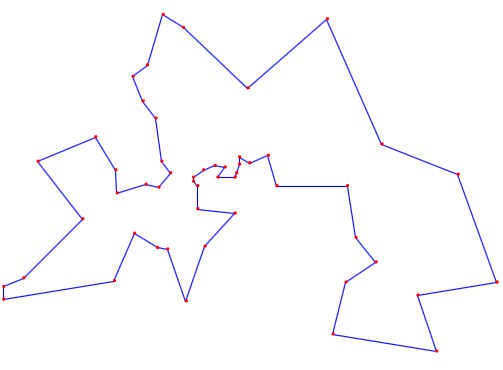
\includegraphics[]{Images/berlin52.png}
	\caption{A solved TSP berlin52 (source: OAT)}
	\label{berlin52}
\end{figure}
\newpage
The algorithmic complexity for a symmetric graph with n nodes is: $\frac{n(n-1)}{2}$ \cite{Applegate}.
The graph is symmetric if the distance between two nodes n and m is the same as the distance between m and n. Asymetric traveling salesman problems also exist with a higher complexity of $n(n-1)$\\
The complexity of the TSP is categorized as non-deterministic polynomial hard (NP-Hard). The runtime of an algorithm can scale exponentially with the number of nodes in the graph and no algorithm is able to solve the problem in polynomial time.\\
Current algorithms work with heuristics to solve the TSP.\\\\
The TSP is common in many real world applications. Drilling of printed circuit boards, computer wiring, order picking in warehouses, vehicle routing and DNA sequencing are some examples \cite{Matai10}.
\section{Mathematical definition}
The symmetric graph is defined as $G=(V,E)$ where $V=\{1,..,n\}$ are the vertices or the nodes and $E=\{(i,j):i,j\in V, i<j\}$ are the edges or routes. Additionally, there is an arc set $A=\{i,j):i,j\in V, i\neq j\}$ which defines all routes in the graph, no route can be used twice. A cost matrix is defined on the edges of the arc set. Usually the cost matrix is calculated using Euclidean distance \cite{Matai10}.\\\\
A typical TSP consists of a set of cities (V), distances between the cities (E) and the cost measured in Euclidean distance between the cities (C). All TSP used in this thesis will follow this convention.\\
The AIS was successfully applied to different TSP by \cite{DEC02} and \cite{RIFF09} This thesis will further examine the performance of an AIS in solving the TSP and which parameters within the AIS are beneficial for a good solution. Furthermore, section \ref{chap:eva} will evaluate under which circumstances AIS are suitable to solve TSP efficiently. The proposed tuning of the CLONALG algorithm by \cite{DEC02} and a modified algorithm, described in section \ref{espc}, will be tested on a wide range of different TSP and two different stopping criteria.
 The next chapter describes the evaluation of the different algorithms and the changes made to them to examine their performance for solving the TSP.


 


